\subsection{Power mode for PSoC 4 moduler}
Alle PSoC 4 moduler besidder fem forskellige power modes: aktiv, sleep, deep-sleep, hibernate og stop. Strømforbruget samt tiden det tager at vågne op fra denne tilstand ses i \figref{fig:Powermode}. 
\begin{figure}[H]
	\centering
	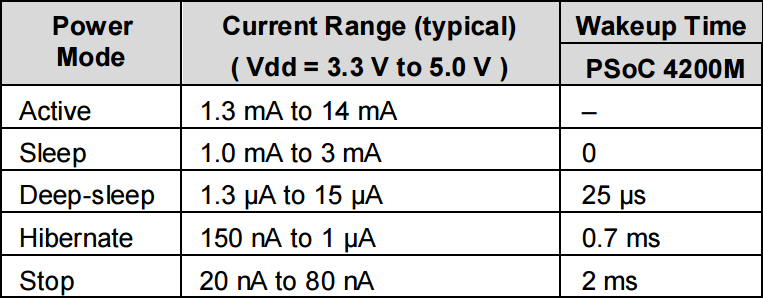
\includegraphics[scale=0.75]{figures/bProblemloesning/PowerMode.jpg}
	\caption{På figuren ses strømforbruget samt opvågningstiden for PSoC 4200M, som er den valgte mikrokontrollers target processor.}
	\label{fig:Powermode}
\end{figure}\vspace{-0.2cm}
Det kan ses på \figref{fig:Powermode}, at hvis der benyttes et batteri til at forsyne mikrokontrolleren, kan det være fordelagtigt, at køre i en lav strømforbrugende tilstand. %Noget med funktionaliteten også afhænger af power moden, fordi nogle ting bliver slukket. Tabel 2 i URL link. Skriv det ind, så det hænger sammen med de andre steder i teksten, hvor der er nævnt noget med dens tilstand.
% http://www.cypress.com/file/121271/download

\subsection{Power mode for LIS331}
% https://cdn.sparkfun.com/assets/learn_tutorials/3/7/3/LSM9DS1_Datasheet.pdf